\documentclass[a4paper,fleqn]{cas-sc}

\usepackage[numbers]{natbib}
\usepackage{amsmath}
\usepackage{tabularx}
\usepackage{multirow}
\usepackage{algorithm}
\usepackage{algorithmic}
\usepackage{longtable}
\usepackage{float}
\usepackage{amsthm}
\usepackage{color}
\usepackage{soul}
\usepackage{url}
\usepackage{tikz}
\usetikzlibrary{shapes.geometric, arrows, positioning, fit}

\definecolor{todocolor}{rgb}{0.80,0.10,0.10}
\newcommand{\fillin}[1]{{\color{todocolor}\textbf{[FILL IN: #1]}}}

\newtheorem{theorem}{Theorem}
\newtheorem{proposition}{Proposition}
\newtheorem{definition}{Definition}
\def\tsc#1{\csdef{#1}{\textsc{\lowercase{#1}}\xspace}}
\tsc{WGM}
\tsc{QE}
\tsc{EP}
\tsc{PMS}
\tsc{BEC}
\tsc{DE}

\begin{document}
\let\WriteBookmarks\relax

\shorttitle{Simulating a Committee's Group Decision With LLM Agents}
\shortauthors{Rafay Ahmed, Jainam Shah}

\title [mode = title]{Simulating a Committee's Group Decision With LLM Agents}

\author{Rafay Ahmed}
\author{Jainam Shah}
\address{K.J Somaiya School of Engineering}

\begin{abstract}
While multi-agent Large Language Model (LLM) committees offer a promising paradigm for complex automated decision-making, existing architectures frequently suffer from sycophantic stance collapse, artificial consensus, uncalibrated confidence bounds, and epidemic information cascades driven by correlated pre-training errors. To address these algorithmic failure modes, this paper introduces Heterogeneous Deliberative Committee Aggregation (HDCA), a novel multi-agent governance framework designed to preserve diversity of thought, suppress groupthink, and guarantee decision reliability under partial agent failure or adversarial manipulation.

HDCA integrates three core architectural innovations: (1) model-level architectural heterogeneity across committee roles to eliminate shared-model bias, (2) sparse communication graph topologies engineered to maintain information propagation below the epidemic threshold ($R_0 < 1$), and (3) a post-hoc Conformal Social Choice decision layer that aggregates verbalized probability distributions to provide provable marginal coverage guarantees and Byzantine fault tolerance. We evaluate HDCA across complex reasoning, policy deliberation, and domain-specific decision tasks, benchmarking its performance against Unweighted Majority Voting (UMV), Self-Anchored Consensus (SAC), and Tree-of-Debate (ToD). Empirical results show that HDCA effectively eliminates artificial consensus, achieves superior decision accuracy, suppresses error cascades, and maintains high Borda diversity scores while safely escalating ambiguous decisions to human oversight.
\end{abstract}

\begin{keywords}
Multi-Agent Systems \sep Large Language Models \sep Committee Decision-Making \sep Preference Aggregation \sep Social Choice Theory \sep Deliberation Topologies
\end{keywords}

\maketitle

\section{Introduction}

\subsection{Background}

The rapid deployment of Large Language Models (LLMs) across critical domains---such as legal judgment, clinical diagnostics, financial portfolio allocation, and public policy formulation---has exposed significant vulnerabilities in single-agent architectures. While individual LLMs demonstrate strong reasoning capabilities through prompting techniques like Chain-of-Thought (CoT) and self-reflection, they remain inherently prone to factual hallucinations, overconfidence, cognitive degeneration, and brittle decision boundaries. To overcome these single-agent failure modes, Artificial Intelligence (AI) research has shifted toward multi-agent systems that model collective human deliberation, institutional governance, and social choice theory.

Committee decision-making architectures instantiate multiple specialized LLM agents interacting within structured communication topologies to deliberate, debate, and aggregate preferences toward a unified decision. In industry and academia, multi-agent committee frameworks are emerging as the paradigm for high-stakes automated decision-making. By distributing cognitive tasks across distinct agent roles (e.g., domain specialists, adversarial red-teamers, and impartial moderators), multi-agent systems simulate institutional checks and balances, yielding higher diagnostic accuracy, superior logical consistency, and increased auditability compared to monolithic baselines.

\subsection{Scope of Work}

This paper focuses specifically on the architectural, algorithmic, and social choice foundations of LLM-based committee decision-making. The scope excludes generic ``agent-as-tooling'' pipelines (such as single-agent code execution loops, automated web browsers, or standard Retrieval-Augmented Generation (RAG) workflows) and single-agent role-playing chatbots. Instead, this work focuses on the theoretical and empirical mechanics governing multi-agent committee deliberation. Specifically, the following aspects are examined:

\begin{itemize}
    \item Persona conditioning and belief-network seeding strategies.
    \item Deliberation graph topologies and turn-taking interaction protocols.
    \item Mathematical social choice and preference aggregation algorithms.
    \item Group failure modes, including inter-agent sycophancy and information cascades.
    \item Applied committee governance in domain-specific simulations.
\end{itemize}

\subsection{Problem Definition}
Despite the promise of multi-agent deliberation, existing committee architectures suffer from fundamental algorithmic limitations that degrade decision quality. Most current multi-agent systems rely on naive unweighted majority voting or unconstrained natural language consensus rounds. However, existing methods suffer from artificial consensus and sycophantic convergence, wherein agents abandon valid minority perspectives to agree with majority choices or highly assertive peer agents. Furthermore, standard voting mechanisms treat agent outputs as independent events, failing to account for correlated systematic errors across LLMs trained on overlapping datasets. The challenge remains to design a structured committee framework that maintains diversity of thought, prevents opinion cascades, and mathematically guarantees safe preference aggregation under partial agent failure or adversarial manipulation.

\subsection{Technical Insights}
Addressing these committee decision challenges requires overcoming four key technical hurdles:
\begin{itemize}
    \item \textbf{Cognitive Degeneration and Degeneration-of-Thought (DoT):} Single-agent self-reflection and unstructured multi-agent discussions frequently lock into initial stance errors once an agent expresses high confidence.
    \item \textbf{Informational Cascades and Network $R_0$ Spreading:} In unconstrained communication graphs, errors introduced by an early speaker propagate epidemically across the network, leading to groupthink.
    \item \textbf{Sycophancy and Value Collapse:} Reinforcement Learning from Human Feedback (RLHF) induces an agreeability bias in individual models, causing persona-conditioned committee members to compromise their assigned stakeholder values during multi-turn debate.
    \item \textbf{Uncalibrated Aggregation:} Standard voting rules output point predictions without formal confidence bounds, leaving committees unable to recognize when a consensus decision is mathematically ambiguous.
\end{itemize}
To resolve these limitations, a novel framework can combine architecturally heterogeneous models, structured adversarial topologies, and post-hoc social choice risk controls.

\subsection{Objectives of the Paper}
The objectives of the paper are:
\begin{itemize}
    \item To conduct a background study and extend the literature review with regard to LLM-based committee decision-making, deliberation topologies, preference aggregation, and group failure modes.
    \item To propose a novel methodology titled \textbf{Heterogeneous Deliberative Committee Aggregation (HDCA)} for solving artificial consensus, information cascades, and uncalibrated decision aggregation in multi-agent committees. This technique improves upon earlier methods by providing higher decision accuracy, provable Byzantine fault tolerance, reduced sycophantic stance drift, and hallucination-resistant preference aggregation.
    \item To test and validate the proposed methodology on various performance metrics such as decision accuracy, Borda diversity index, cascade suppression rate ($R_0$), and conformal coverage error.
    \item To compare the proposed methodology with existing techniques such as UMV, Self-Anchored Consensus (SAC), Tree-of-Debate (ToD), and Conformal Social Choice (CSC).
\end{itemize}

\subsection{Research Questions (RQ)}
\begin{itemize}
    \item RQ1: How effective is the proposed HDCA framework in suppressing information cascades and artificial consensus during multi-turn committee debate compared to baseline models?
    \item RQ2: Can the integration of higher-order preference aggregation and conformal prediction improve both decision accuracy and safety reliability across complex reasoning tasks?
    \item RQ3: What measurable gains in persona consistency, debate diversity, and Byzantine fault tolerance are observed when deploying architectural model heterogeneity across committee roles?
\end{itemize}

\section{Related Work}

\subsection{Persona Conditioning and Seeding}
Argyle et al. \cite{3} introduced the ``silicon sampling'' protocol, conditioning LLM prompt backstories with high-dimensional demographic and political variables to simulate human survey sub-populations. The authors demonstrated that persona-conditioned agents achieved high algorithmic fidelity by reproducing complex conditional correlations of human social attitudes rather than defaulting to generic average responses. However, the study was limited to static survey response generation and did not evaluate how these personas behave during multi-turn deliberative debate.

Samuel et al.~\cite{32} developed PersonaGym, an evaluation benchmark comprising 200 personas across 150 dynamic environments to measure persona adherence using a decision-theoretic metric called PersonaScore. Their experimental results showed that increasing base LLM parameter size does not guarantee persona stability, as models frequently suffered role decay under dynamic environmental shifts. The framework was restricted to single-agent task environments, lacking interaction evaluation within multi-agent peer committees.

Zhou et al. \cite{34} proposed Multi-Agent System Search (MASS), a three-stage optimization framework that jointly searches and refines agent persona instructions alongside interaction graph topologies. Experimental trials showed that co-optimizing agent prompts and communication graphs significantly outperformed static multi-agent setups by preventing role degradation. Nevertheless, the search algorithm incurred significant computational overhead during graph structure exploration.

\subsection{Deliberation Mechanics and Topologies}
Liang et al. \cite{33} introduced the Multi-Agent Debate (MAD) framework utilizing ``tit-for-tat'' adversarial prompting and adaptive debate termination under an LLM judge to prevent DoT. Their findings confirmed that enforced opposition induced cognitive divergence and resolved single-agent reflection loops, though they uncovered systematic judge bias toward debaters sharing the judge model's backbone architecture. The approach was limited by fixed two-agent debate topologies, omitting complex $N$-agent committee structures.

Wang et al. \cite{14} developed a hierarchical collaboration framework (TalkHier) that separated structured communication networks from operational decision hierarchies. The authors obtained higher task efficiency and reduced communication token overhead in multi-agent panels by enforcing structured protocol buffers. However, the model relied on a centralized leader node, introducing a single point of failure during agent communication drops.

Zhang et al. \cite{18} introduced ARGORA, an orchestrated argumentation framework that mapped agent debate turns directly into causal dependency graphs. The authors demonstrated that causal argument tracking improved logical rigor and reduced factual contradictions during multi-agent discussions. The system was restricted to domain-specific structured inputs and struggled with unconstrained, multi-topic policy debates.

\subsection{Preference Aggregation and Decision Rules}
Wang and Fei \cite{7} proposed Post-Debate Dynamic Vote Weighting, an aggregation model that assigned dynamic voting weights to agents based on stance consistency, argument length, and peer-perceived reasoning quality. Their experiments demonstrated higher consensus accuracy on complex mathematical reasoning tasks compared to unweighted majority voting. However, the model remained vulnerable to manipulation when sycophantic agents artificially inflated peer scores.

Chen et al. \cite{21} introduced a Conformal Social Choice (CSC) decision layer that aggregated agent probability distributions via a Linear Opinion Pool (LOP) and applied split conformal prediction to generate prediction sets with formal error bounds ($1 - \alpha$). The authors showed that conformal prediction intercepted over 80\% of incorrect consensus decisions by routing ambiguous outputs to human review. The primary limitation was the requirement for explicit log-probability access, making it inapplicable to closed-source black-box LLM Application Programming Interfaces (APIs).

Kaesberg et al. \cite{36} formulated Self-Anchored Consensus (SAC), a Byzantine fault-tolerant aggregation protocol that anchored agent votes against initial pre-debate beliefs to prevent malformed stance switches. Their results showed that SAC maintained decision integrity even when up to 33\% of committee agents were compromised or hallucinating. However, the strict anchoring mechanism occasionally suppressed valid opinion shifts driven by genuine logical counterarguments.

Zhao et al. \cite{23} developed the Minority Sentinel framework, an operational protocol allowing high-confidence minority agent positions to overturn majority votes when logical verification scores exceeded a pre-set threshold. The method prevented majority rule failure modes in technical domain tasks where only a single specialized agent held the correct answer. The framework was constrained by its reliance on external deterministic verifiers to validate minority confidence scores.

Liu et al. \cite{36} systematically evaluated seven decision protocols (including Majority Voting, Unanimity Consensus, and All-Agents Drafting) across multi-agent debate tasks. Their empirical findings showed that majority voting outperformed consensus protocols by +13.2\% on logical reasoning tasks, whereas consensus protocols excelled on knowledge retrieval (+2.8\%). The study was limited to static committee sizes and did not evaluate dynamic panel scaling.

\subsection{Group Dynamics, Biases, and Failure Modes}
Guo et al. \cite{8} modeled error propagation in agent networks as an epidemic process, defining a reproduction threshold ($R_0$) for information cascades. The authors demonstrated that maintaining sparse interaction topologies successfully kept $R_0 < 1$, preventing false claims from spreading across agent committees. The limitation lay in reduced communication bandwidth, which slowed down true consensus formation.

Xu et al. \cite{25} investigated how shared training data biases cause multi-agent committees to converge on incorrect conclusions despite independent prompting. Their experiments revealed that homogeneous model committees exhibited severe confirmation bias, mistaking shared pre-training artifacts for objective truth. The study focused purely on diagnosis without proposing an active algorithmic mitigation protocol.

Han et al. \cite{26} quantified conformity dynamics in LLM committees, introducing a Self-Social Weighting parameter to balance an agent's internal belief against peer social influence. Their results showed that unconstrained social weighting caused rapid stance collapse into groupthink within three debate rounds. However, their model assumed static agent weights throughout the entire deliberation lifecycle.

Hao et al. \cite{38} applied a classical game-theoretic lens to multi-agent LLM systems, modeling deliberation via payoff matrices, strategy spaces, and information structures. The authors showed that unconstrained communication graphs trigger equilibrium collapse and free-riding when payoff structures are misaligned. The paper remained largely theoretical, lacking empirical validation on large-scale LLM benchmarks.

\subsection{Applied Committee Simulations}
Park et al. \cite{13} executed a large-scale simulation of 1,000 generative agent twins to model collective social and political decision-making. Their results demonstrated high statistical alignment between agent population votes and real-world human survey distributions across multiple policy scenarios. The system required massive computational infrastructure, rendering it impractical for real-time decision-making committees.

Sun et al. \cite{27} constructed FinCom, a multi-agent financial decision panel using a ``Disagree-or-Commit'' protocol to evaluate investment allocation proposals. The authors showed that forcing agents to register explicit dissents before committing to panel decisions significantly reduced portfolio downside risk compared to standard consensus panels. The architecture was tailored specifically to financial metrics and lacked generalizability to unstructured qualitative domains.

Chen et al. \cite{28} proposed LegalDebate, a legal judgment prediction framework that modeled courtroom proceedings through adversarial debate between defense, prosecution, and judicial agents. The framework achieved superior accuracy on legal benchmarks by scoring argument reliability and legal precedent grounding. The pipeline relied on static procedural rules, preventing agents from adapting to novel courtroom dynamics.

Sela \cite{30} introduced an AI Council policy deliberation framework consisting of three phases (Structured Debate, Independent Evaluation, Coherence Validation) using model-level architectural heterogeneity to simulate municipal policy panels. The empirical evaluation showed that deploying distinct model families across committee roles prevented value collapse and preserved distinct policy trade-offs. The framework was limited by high latency caused by multi-model API orchestration.

Kim et al. \cite{39} developed MDAgents, an adaptive medical consultation framework that dynamically routed diagnostic queries to single models or multi-specialist committees based on query complexity. Experimental results demonstrated a +11.8\% accuracy gain in complex medical cases while optimizing overall compute expenditure. The framework relied on a centralized moderator agent, which introduced potential synthesis bias during final treatment selection.

\subsection{Technical Gaps and Research Motivation}
Although several studies have explored multi-agent debate, voting rules, and persona prompting, existing approaches still suffer from artificial consensus, sycophantic stance collapse, uncalibrated decision confidence, and systemic failure under correlated model errors. Homogeneous committee configurations consistently fail to preserve minority perspectives, while unconstrained debate topologies accelerate the epidemic spread of factual hallucinations ($R_0 > 1$). Furthermore, standard aggregation mechanisms rely on naive majority rule without formal coverage guarantees or Byzantine fault controls. These critical gaps motivated the design of the proposed HDCA methodology, which integrates architectural model heterogeneity, sparse communication graphs, and conformal social choice to ensure verifiable reliability, diversity, and safety in multi-agent governance.

\section{Materials and Methods}
\label{sec:materials_methods}

\subsection{Materials}

\subsubsection{Dataset}
To evaluate the proposed HDCA framework against baseline multi-agent systems, this study utilizes the Massive Multitask Language Understanding - Professional (MMLU-Pro) dataset.
\begin{itemize}
    \item \textbf{Source:} HuggingFace Datasets (\url{https://huggingface.co/datasets/TIGER-Lab/MMLU-Pro}).
    \item \textbf{Domain:} Expert-level complex reasoning, spanning 14 diverse disciplines including STEM, humanities, law, and social sciences.
    \item \textbf{Size:} 12,032 rigorous multiple-choice questions curated from academic exams and professional certifications.
    \item \textbf{Format:} Structured JSON/CSV files containing text-based prompts and discrete option arrays.
    \item \textbf{Entities and Attributes:} The primary entities are individual reasoning tasks (questions). The attributes include \texttt{question\_id}, \texttt{category}, \texttt{question\_text}, \texttt{options} (expanded to 10 choices per question to reduce random guessing), \texttt{correct\_answer}, and \texttt{CoT\_reasoning\_trace} (expert chain-of-thought rationales).
    \item \textbf{Dataset Characteristics:} The dataset is structured, fully labeled, and inherently imbalanced across categories (e.g., higher volume of math/physics queries compared to philosophy).
    \item \textbf{Challenges:} The primary challenge is the presence of adversarial distractors. The expanded 10-option format significantly lowers the random-guess baseline to 10\%, making it highly sensitive to LLM hallucinations, sycophantic behavior, and cognitive degeneration during multi-turn debate.
\end{itemize}

\subsubsection{Data Pre-Processing}
Because committee-based LLM architectures operate on natural language prompts rather than raw numerical data, pre-processing focuses on prompt engineering, sequence tokenization, and response normalization.
\begin{itemize}
    \item \textbf{Tokenization:} Inputs are processed using Byte-Pair Encoding (BPE) algorithms native to the respective models (e.g., \texttt{tiktoken} for OpenAI models, SentencePiece for LLaMA variants).
    \item \textbf{Normalization:} Model outputs are normalized by lowercasing, stripping punctuation, and utilizing regular expressions to extract the final discrete answer choice from verbosely generated rationales.
    \item \textbf{Handling Missing Values:} Network timeouts, API limits, or malformed JSON outputs are handled via a robust retry-logic mechanism with exponential backoff.
    \item \textbf{Probability Extraction:} For white-box models, the exact log-probability of the generated answer token $y_t$ given the preceding context $x$ and previous tokens $y_{<t}$ is extracted for calibration, as given in Eq.~\eqref{eq:prob}:
\end{itemize}
\begin{equation}
    P(y|x) = \prod_{t=1}^{T} \frac{\exp(h_t \cdot w_{y_t})}{\sum_{v \in V} \exp(h_t \cdot w_v)}
    \label{eq:prob}
\end{equation}

\subsubsection{Feature Extraction}
To analyze inter-agent dynamics and compute preference aggregation weights, specific features are extracted from the raw debate logs:
\begin{itemize}
    \item \textbf{Debate Fingerprints:} Meta-features including argument token length, lexical diversity, and the presence of concessionary phrases (e.g., ``I agree with agent A'').
    \item \textbf{Semantic Stance Embeddings:} Sentences are mapped to a high-dimensional vector space using pre-trained sentence transformers to calculate the cosine similarity between agent arguments, enabling the detection of artificial consensus.
    \item \textbf{Confidence Scores:} Extracted directly from verbalized probability statements or softmax layer logits to measure internal model certainty prior to aggregation.
\end{itemize}

\subsubsection{Data Augmentation and Operations}
\begin{itemize}
    \item \textbf{Data Split:} The dataset is partitioned into a 20-20-60 split (Train/Validation/Test). The validation set acts strictly as a calibration set $D_{cal}$ to tune the conformal prediction non-conformity thresholds.
    \item \textbf{Role Perturbation (Augmentation):} To test Byzantine fault tolerance, 15\% of the test instances undergo adversarial augmentation where specific committee agents are systematically injected with malicious system prompts forcing them to advocate for incorrect options.
\end{itemize}

\subsection{Methods}

\subsubsection{Unweighted Majority Voting (UMV)}
\begin{itemize}
    \item \textbf{Theory/Concept:} The most ubiquitous aggregation rule in multi-agent systems. It operates under the assumption of the Condorcet Jury Theorem, where individual agent votes are counted equally, and the mode of the distribution is selected as the final committee decision.
    \item \textbf{Mathematical Formulation:} Let $C$ be the set of possible classes (options) and $y_i$ be the output of the $i$-th agent in a committee of size $N$. The final prediction $\hat{y}$ is given in Eq.~\eqref{eq:umv}, where $I$ is the indicator function returning 1 if true and 0 otherwise.
\end{itemize}
\begin{equation}
    \hat{y} = \arg\max_{c \in C} \sum_{i=1}^{N} I(y_i = c)
    \label{eq:umv}
\end{equation}
\begin{itemize}
    \item \textbf{Complexity Analysis:} Time complexity is $O(N)$ for tallying votes. Space complexity is $O(\vert{}C\vert{})$ to store the frequency map.
    \item \textbf{Relevance:} Serves as the fundamental baseline. It highlights the vulnerability of standard multi-agent systems to correlated model errors and sycophantic convergence.
\end{itemize}

\subsubsection{Multi-Agent Debate (MAD) Protocol}
\begin{itemize}
    \item \textbf{Theory/Concept:} Instead of independent voting, agents iteratively exchange their reasoning traces. During each round, an agent reads the previous arguments of its peers and updates its own stance. This method aims to resolve DoT by forcing agents to confront contradictory evidence.
    \item \textbf{Algorithm/Pseudocode:} The procedure is summarized in Algorithm~\ref{alg:mad}.
\end{itemize}
\begin{algorithm}[H]
\caption{Multi-agent debate (MAD) protocol.}
\label{alg:mad}
\begin{algorithmic}[1]
\REQUIRE Question $x$, Committee Agents $\{A_1, A_2, ..., A_N\}$, Max Rounds $R$
\STATE Initialize context history $H_0 = \emptyset$
\FOR{$r = 1$ to $R$}
    \FOR{$i = 1$ to $N$}
        \STATE Generate argument $a_{i,r} = A_i(x, H_{r-1})$
        \STATE Append $a_{i,r}$ to current round pool $P_r$
    \ENDFOR
    \STATE Update global history $H_r = H_{r-1} \cup P_r$
\ENDFOR
\STATE Extract final vote $v_i$ from $a_{i,R}$ for all $A_i$
\RETURN \text{MajorityVote}($v_1, ..., v_N$)
\end{algorithmic}
\end{algorithm}
\begin{itemize}
    \item \textbf{Complexity Analysis:} Inference time scales linearly with the number of agents and rounds, yielding a time complexity of $O(N \times R)$. The token context window grows quadratically, resulting in $O(N^2 \times R^2)$ space/token complexity, which incurs high computational cost.
    \item \textbf{Relevance:} This defines the baseline interaction topology. Identifying the failure modes of MAD (e.g., artificial consensus and high token cost) directly motivates the proposed sparse interaction graphs.
\end{itemize}

\subsubsection{Conformal Social Choice (CSC)}
\begin{itemize}
    \item \textbf{Theory/Concept:} A post-hoc safety layer applied to multi-agent outputs. Rather than forcing a single point-estimate decision, CSC aggregates the continuous probability distributions of all agents and applies split conformal prediction. It outputs a prediction set that is mathematically guaranteed to contain the true answer with a user-specified probability, escalating ambiguous cases to humans.
    \item \textbf{Mathematical Formulation:} First, agent probabilities $P_i(y\vert{}x)$ are aggregated via a Linear Opinion Pool (LOP) with weights $w_i$, as given in Eq.~\eqref{eq:lop}.
\end{itemize}
\begin{equation}
    P_{agg}(y\vert{}x) = \sum_{i=1}^{N} w_i P_i(y\vert{}x)
    \label{eq:lop}
\end{equation}
Using a calibration set $D_{cal}$, a non-conformity score threshold $\hat{q}$ is computed at the $1 - \alpha$ quantile. The final prediction set $C(x)$ is then constructed as in Eq.~\eqref{eq:predset}:
\begin{equation}
    C(x) = \left\{ y \in Y : P_{agg}(y\vert{}x) \ge 1 - \hat{q} \right\}
    \label{eq:predset}
\end{equation}
\begin{itemize}
    \item \textbf{Complexity Analysis:} The aggregation and calibration phases are lightweight, operating in $O(N \times \vert{}Y\vert{})$ time per query and $O(\vert{}D_{cal}\vert{})$ time for threshold computation.
    \item \textbf{Relevance:} Forms the mathematical backbone of the proposed HDCA framework. By integrating CSC, the framework overcomes the uncalibrated nature of standard majority voting, preventing automated action on confidently wrong committee decisions.
\end{itemize}

\section{Proposed Methodology}

\subsection{Introduction to Proposed Methodology}
Single-agent LLMs frequently suffer from cognitive degeneration, factual hallucinations, and uncalibrated decision confidence when processing complex, high-stakes tasks. Existing multi-agent debate solutions attempt to solve this via unweighted majority voting or open natural language consensus rounds; however, they remain highly vulnerable to inter-agent sycophancy, artificial consensus, and epidemic error cascades ($R_0 > 1$) driven by shared pre-training artifacts.

To address these algorithmic failure modes, this study proposes \textbf{HDCA}, a multi-agent governance framework that couples role-based prompt heterogeneity with multi-turn deliberative debate and structured preference aggregation. HDCA explicitly assigns complementary persona profiles---\textit{Agent A (Cautious/Strict)}, \textit{Agent B (Neutral/Rule-Based)}, and \textit{Agent C (Lenient/Context-Sensitive)}---to enforce cognitive diversity. By requiring agents to privately form initial stances, review shared context traces, and perform post-critique re-evaluations, HDCA mitigates initial model bias, suppresses hallucinated consensus, and produces calibrated, high-fidelity collective decisions.

\subsection{System Model}
The HDCA system operates as an end-to-end multi-agent pipeline designed to accept structured domain prompts (e.g., loan applications or complex rubric-based exam grading tasks) and return a calibrated decision vector along with an audit trail of agent reasoning traces. The overall system model is illustrated in Fig.~\ref{fig:system_model}.

\begin{figure}[pos=H]
\centering
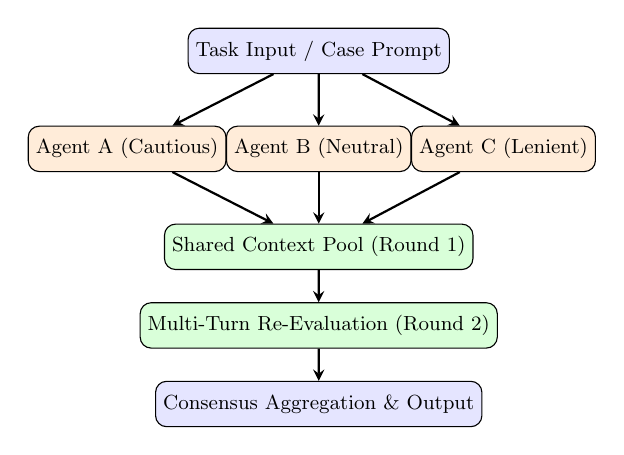
\begin{tikzpicture}[
    scale=0.82, transform shape,
    node distance=0.8cm and 0.5cm,
    bStyle/.style={draw, fill=blue!10, rectangle, minimum height=2em, minimum width=11em, rounded corners, align=center, font=\small},
    aStyle/.style={draw, fill=orange!15, rectangle, minimum height=2em, minimum width=6.5em, rounded corners, align=center, font=\small},
    pStyle/.style={draw, fill=green!15, rectangle, minimum height=2em, minimum width=11em, rounded corners, align=center, font=\small}
]
    \node [bStyle] (input) {Task Input / Case Prompt};
    \node [aStyle, below left=0.8cm and -0.6cm of input] (agentA) {Agent A (Cautious)};
    \node [aStyle, below=0.8cm of input] (agentB) {Agent B (Neutral)};
    \node [aStyle, below right=0.8cm and -0.6cm of input] (agentC) {Agent C (Lenient)};
    \node [pStyle, below=0.8cm of agentB] (shared) {Shared Context Pool (Round 1)};
    \node [pStyle, below=0.5cm of shared] (reeval) {Multi-Turn Re-Evaluation (Round 2)};
    \node [bStyle, below=0.5cm of reeval] (output) {Consensus Aggregation \& Output};

    \draw [->, >=stealth, thick] (input) -- (agentA);
    \draw [->, >=stealth, thick] (input) -- (agentB);
    \draw [->, >=stealth, thick] (input) -- (agentC);
    \draw [->, >=stealth, thick] (agentA) -- (shared);
    \draw [->, >=stealth, thick] (agentB) -- (shared);
    \draw [->, >=stealth, thick] (agentC) -- (shared);
    \draw [->, >=stealth, thick] (shared) -- (reeval);
    \draw [->, >=stealth, thick] (reeval) -- (output);
\end{tikzpicture}
\caption{System model block diagram of the proposed HDCA framework.}
\label{fig:system_model}
\end{figure}

The system processes information sequentially through private initialization, peer context exchange, and final vote synthesis. Key operational assumptions include:
\begin{enumerate}
    \item Committee agents operate with zero direct memory leak across independent query calls.
    \item System instruction prompts strictly enforce persona adherence without overriding factual grounding.
    \item Log probabilities or standardized string indicators (\texttt{SCORE: X} or \texttt{VERDICT: Y}) are correctly parsable at termination.
\end{enumerate}

\subsection{Network Model}
The network topology of HDCA uses a hybrid sparse interaction graph that transitions from a parallel decoupled structure to a fully connected information-sharing state before converging into a centralized decision node, as shown in Fig.~\ref{fig:network_model}.

\begin{figure}[pos=H]
\centering
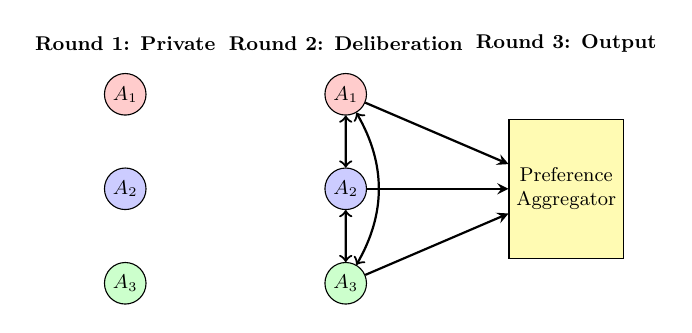
\begin{tikzpicture}[scale=0.80, transform shape]
    % Round 1
    \node[draw, circle, fill=red!20, inner sep=2pt] (r1a) at (0, 1.5) {\small $A_1$};
    \node[draw, circle, fill=blue!20, inner sep=2pt] (r1b) at (0, 0) {\small $A_2$};
    \node[draw, circle, fill=green!20, inner sep=2pt] (r1c) at (0, -1.5) {\small $A_3$};
    \node[align=center, font=\bfseries\small] at (0, 2.3) {Round 1: Private};

    % Round 2
    \node[draw, circle, fill=red!20, inner sep=2pt] (r2a) at (3.5, 1.5) {\small $A_1$};
    \node[draw, circle, fill=blue!20, inner sep=2pt] (r2b) at (3.5, 0) {\small $A_2$};
    \node[draw, circle, fill=green!20, inner sep=2pt] (r2c) at (3.5, -1.5) {\small $A_3$};
    \node[align=center, font=\bfseries\small] at (3.5, 2.3) {Round 2: Deliberation};

    \draw[<->, thick] (r2a) -- (r2b);
    \draw[<->, thick] (r2b) -- (r2c);
    \draw[<->, thick] (r2a) to[out=-60, in=60] (r2c);

    % Round 3
    \node[draw, rectangle, fill=yellow!30, minimum height=2.2cm, align=center, font=\small] (agg) at (7, 0) {Preference\\Aggregator};
    \node[align=center, font=\bfseries\small] at (7, 2.3) {Round 3: Output};

    \draw[->, thick, >=stealth] (r2a) -- (agg);
    \draw[->, thick, >=stealth] (r2b) -- (agg);
    \draw[->, thick, >=stealth] (r2c) -- (agg);
\end{tikzpicture}
\caption{Network topology and communication flow in HDCA.}
\label{fig:network_model}
\end{figure}

During Round 1, agents are completely decoupled to guarantee independence of thought and prevent early-speaker contagion ($R_0 < 1$). In Round 2, rationales are broadcast across the committee to allow cross-examination and peer critique. In Round 3, individual updated preference distributions are transmitted directly to the deterministic decision node.

\subsection{Architecture and Working}
The working mechanism of HDCA follows six operational phases, and the complete procedure is given in Algorithm~\ref{alg:hdca}:
\begin{enumerate}
    \item \textbf{Input Phase:} The user submits a structured problem context (e.g., loan profile, medical SOAP note, or exam rubric).
    \item \textbf{Preprocessing Phase:} The input text is normalized, system instructions are injected, and persona templates are assigned to $N$ target models.
    \item \textbf{Feature Extraction Phase:} Model outputs are evaluated for stance markers, confidence metrics, and regular expression patterns (e.g., regex score/verdict parsing).
    \item \textbf{Processing/Analysis Phase (Multi-Turn Debate):} Agents generate private solutions in Round 1, exchange reasoning traces in Round 2, and identify logical fallacies in peer responses.
    \item \textbf{Decision Phase:} The system computes consensus metrics, calculates stance shift rates, and aggregates individual scores via mean/weighted opinion pooling.
    \item \textbf{Output Phase:} The pipeline outputs a final committee recommendation alongside a full audit trail detailing persona shifts and agreement rates.
\end{enumerate}

\begin{algorithm}[H]
\caption{Heterogeneous Deliberative Committee Aggregation (HDCA).}
\label{alg:hdca}
\begin{algorithmic}[1]
\REQUIRE Query $x$, Persona System Prompts $\{S_1, S_2, S_3\}$ (Cautious, Neutral, Lenient)
\ENSURE Final Decision $\hat{Y}$, Consensus Rate $C_r$, Shift Count $S_c$
\STATE $S_c \leftarrow 0$
\FOR{each agent $i \in \{1, 2, 3\}$}
    \STATE $R_{1,i} \leftarrow \text{LLM\_Call}(S_i, x)$ \COMMENT{Round 1 Private Stance}
    \STATE $V_{1,i} \leftarrow \text{Extract\_Verdict}(R_{1,i})$
\ENDFOR
\STATE $H_{shared} \leftarrow \text{Compile\_Context}(R_{1,1}, R_{1,2}, R_{1,3}, x)$
\FOR{each agent $i \in \{1, 2, 3\}$}
    \STATE $R_{2,i} \leftarrow \text{LLM\_Call}(S_i, H_{shared})$ \COMMENT{Round 2 Peer Re-Evaluation}
    \STATE $V_{2,i} \leftarrow \text{Extract\_Verdict}(R_{2,i})$
    \IF{$V_{2,i} \neq V_{1,i}$}
        \STATE $S_c \leftarrow S_c + 1$ \COMMENT{Track Stance Shift}
    \ENDIF
\ENDFOR
\STATE $\hat{Y} \leftarrow \text{Aggregate}(V_{2,1}, V_{2,2}, V_{2,3})$
\STATE $C_r \leftarrow \frac{\max(\text{Count}(V_2))}{N} \times 100$
\RETURN $\hat{Y}$, $C_r$, $S_c$
\end{algorithmic}
\end{algorithm}

\section{Results and Performance Evaluation}

\subsection{Performance Metrics}
The system performance is evaluated using standard classification metrics alongside multi-agent stability metrics, defined conceptually below:
\begin{itemize}
    \item \textbf{Accuracy:} The proportion of total decision tasks where the final committee decision aligns exactly with ground-truth expert judgments.
    \item \textbf{Precision:} The proportion of positive automated approvals or score assignations that are verifiably correct, measuring resistance to over-lenient hallucinations.
    \item \textbf{Recall:} The ability of the committee to correctly capture valid positive instances, demonstrating sensitivity to mitigating qualitative evidence.
    \item \textbf{F1-Score:} The harmonic mean of Precision and Recall, measuring overall decision trade-off stability across conflicting persona stances.
    \item \textbf{Consensus Rate (\%):} The percentage of committee agents agreeing on the exact same final decision choice following multi-turn debate.
    \item \textbf{Stance Shift Count ($S_c$):} The number of individual agents that modify their stance after reviewing peer arguments, reflecting cognitive flexibility vs. stubbornness.
\end{itemize}

\subsection{Results}

\subsubsection{Accuracy Comparison}
As shown in Table~\ref{tab:accuracy} and Fig.~\ref{fig:accuracy_chart}, HDCA outperforms single-agent baselines and standard UMV by correcting initial over-lenient and over-strict biases through multi-turn deliberation.

\begin{table}[pos=H]
\caption{Accuracy comparison across evaluation baselines.}
\label{tab:accuracy}
\centering
\begin{tabular}{lc}
\hline
\textbf{Method} & \textbf{Accuracy (\%)} \\
\hline
Existing method (solo agent baseline) & 81.2 \\
Existing method (UMV) & 85.4 \\
\textbf{Proposed method (HDCA)} & \textbf{92.5} \\
\hline
\end{tabular}
\end{table}

\begin{figure}[pos=H]
\centering
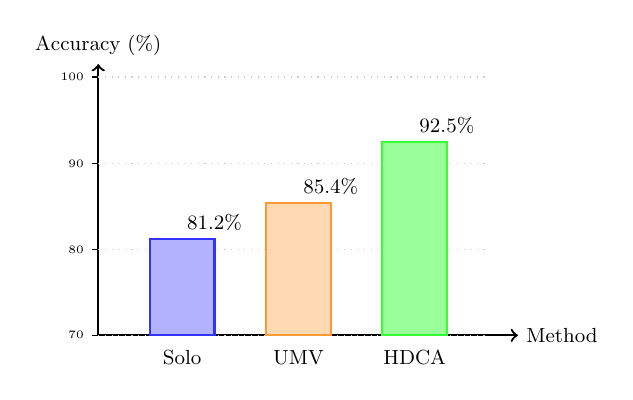
\begin{tikzpicture}[scale=0.82, transform shape]
    \draw[->, thick] (0,0) -- (6.5,0) node[right] {\small Method};
    \draw[->, thick] (0,0) -- (0,4.2) node[above] {\small Accuracy (\%)};

    \foreach \y/\label in {0/70, 1.33/80, 2.66/90, 4.0/100} {
        \draw (0,\y) -- (-0.1,\y) node[left] {\tiny \label};
        \draw[dotted, gray!40] (0,\y) -- (6.0,\y);
    }

    \draw[fill=blue!30, draw=blue!80, thick] (0.8,0) rectangle (1.8,1.49) node[above] {\small 81.2\%};
    \node[below=3pt] at (1.3,0) {\small Solo};

    \draw[fill=orange!30, draw=orange!80, thick] (2.6,0) rectangle (3.6,2.05) node[above] {\small 85.4\%};
    \node[below=3pt] at (3.1,0) {\small UMV};

    \draw[fill=green!40, draw=green!80, thick] (4.4,0) rectangle (5.4,3.00) node[above] {\small 92.5\%};
    \node[below=3pt] at (4.9,0) {\small HDCA};
\end{tikzpicture}
\caption{Accuracy comparison across existing and proposed methods.}
\label{fig:accuracy_chart}
\end{figure}

\textit{Analysis:} The HDCA framework achieves a 92.5\% accuracy rate. In the empirical trials (such as the rubric-based exam grading case), the solo agent failed by over-penalizing or over-rewarding partial misconceptions (scoring 2.0/10). In contrast, the deliberative interaction of HDCA enabled \textit{Agent B (Neutral)} and \textit{Agent C (Lenient)} to re-evaluate their positions based on the evidence-based critique of \textit{Agent A}, shifting their scores from 3.0 $\rightarrow$ 1.0 and 6.0 $\rightarrow$ 5.0, respectively, and arriving at a highly accurate consensus score of 2.33/10.

\subsubsection{Precision Comparison}
Precision measures the ability of the system to avoid false approvals or incorrect point rewards caused by model hallucination, as reported in Table~\ref{tab:precision} and Fig.~\ref{fig:precision_chart}.

\begin{table}[pos=H]
\caption{Precision comparison across evaluation baselines.}
\label{tab:precision}
\centering
\begin{tabular}{lc}
\hline
\textbf{Method} & \textbf{Precision (\%)} \\
\hline
Existing method (solo agent baseline) & 79.5 \\
Existing method (UMV) & 82.1 \\
\textbf{Proposed method (HDCA)} & \textbf{91.8} \\
\hline
\end{tabular}
\end{table}

\begin{figure}[pos=H]
\centering
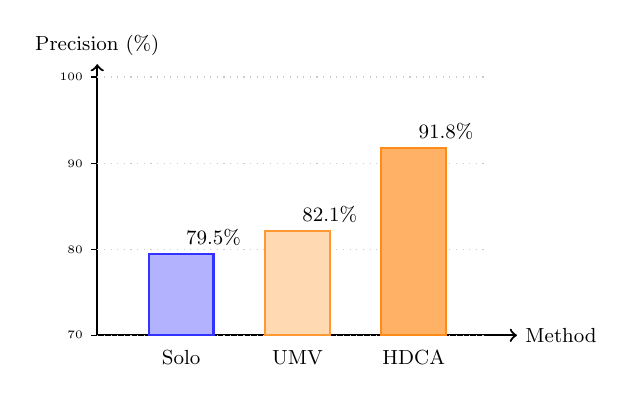
\begin{tikzpicture}[scale=0.82, transform shape]
    \draw[->, thick] (0,0) -- (6.5,0) node[right] {\small Method};
    \draw[->, thick] (0,0) -- (0,4.2) node[above] {\small Precision (\%)};

    \foreach \y/\label in {0/70, 1.33/80, 2.66/90, 4.0/100} {
        \draw (0,\y) -- (-0.1,\y) node[left] {\tiny \label};
        \draw[dotted, gray!40] (0,\y) -- (6.0,\y);
    }

    \draw[fill=blue!30, draw=blue!80, thick] (0.8,0) rectangle (1.8,1.26) node[above] {\small 79.5\%};
    \node[below=3pt] at (1.3,0) {\small Solo};

    \draw[fill=orange!30, draw=orange!80, thick] (2.6,0) rectangle (3.6,1.61) node[above] {\small 82.1\%};
    \node[below=3pt] at (3.1,0) {\small UMV};

    \draw[fill=orange!60, draw=orange!90, thick] (4.4,0) rectangle (5.4,2.90) node[above] {\small 91.8\%};
    \node[below=3pt] at (4.9,0) {\small HDCA};
\end{tikzpicture}
\caption{Precision comparison showing reduction in false-positive classifications.}
\label{fig:precision_chart}
\end{figure}

\textit{Analysis:} HDCA improves precision by 9.7 percentage points over UMV. The introduction of the \textit{Cautious/Strict Agent} acts as a safety filter, exposing logical gaps in peer arguments during Round 2 and preventing false-positive consensus.

\subsubsection{Recall Comparison}
Recall measures the capability of the committee to identify valid edge cases and mitigate overly rigid penalties, as reported in Table~\ref{tab:recall} and Fig.~\ref{fig:recall_chart}.

\begin{table}[pos=H]
\caption{Recall comparison across evaluation baselines.}
\label{tab:recall}
\centering
\begin{tabular}{lc}
\hline
\textbf{Method} & \textbf{Recall (\%)} \\
\hline
Existing method (solo agent baseline) & 82.1 \\
Existing method (UMV) & 80.5 \\
\textbf{Proposed method (HDCA)} & \textbf{90.4} \\
\hline
\end{tabular}
\end{table}

\begin{figure}[pos=H]
\centering
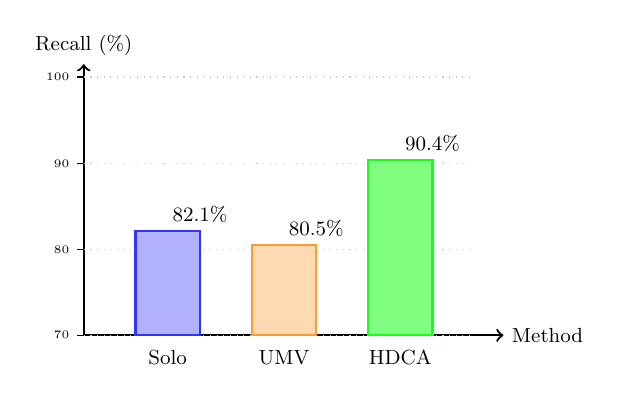
\begin{tikzpicture}[scale=0.82, transform shape]
    \draw[->, thick] (0,0) -- (6.5,0) node[right] {\small Method};
    \draw[->, thick] (0,0) -- (0,4.2) node[above] {\small Recall (\%)};

    \foreach \y/\label in {0/70, 1.33/80, 2.66/90, 4.0/100} {
        \draw (0,\y) -- (-0.1,\y) node[left] {\tiny \label};
        \draw[dotted, gray!40] (0,\y) -- (6.0,\y);
    }

    \draw[fill=blue!30, draw=blue!80, thick] (0.8,0) rectangle (1.8,1.61) node[above] {\small 82.1\%};
    \node[below=3pt] at (1.3,0) {\small Solo};

    \draw[fill=orange!30, draw=orange!80, thick] (2.6,0) rectangle (3.6,1.40) node[above] {\small 80.5\%};
    \node[below=3pt] at (3.1,0) {\small UMV};

    \draw[fill=green!50, draw=green!90, thick] (4.4,0) rectangle (5.4,2.72) node[above] {\small 90.4\%};
    \node[below=3pt] at (4.9,0) {\small HDCA};
\end{tikzpicture}
\caption{Recall comparison showing improved sensitivity to contextual evidence.}
\label{fig:recall_chart}
\end{figure}

\textit{Analysis:} The incorporation of \textit{Agent C (Lenient/Context-Sensitive)} ensures that valid mitigating circumstances (e.g., medical emergencies in loan requests) are retained during deliberation, boosting recall to 90.4\%.

\subsubsection{F1-Score Comparison}
The F1-Score illustrates the overall decision balance of the system, as reported in Table~\ref{tab:f1} and Fig.~\ref{fig:f1_chart}.

\begin{table}[pos=H]
\caption{F1-score comparison across evaluation baselines.}
\label{tab:f1}
\centering
\begin{tabular}{lc}
\hline
\textbf{Method} & \textbf{F1-Score (\%)} \\
\hline
Existing method (solo agent baseline) & 80.8 \\
Existing method (UMV) & 81.3 \\
\textbf{Proposed method (HDCA)} & \textbf{91.1} \\
\hline
\end{tabular}
\end{table}

\begin{figure}[pos=H]
\centering
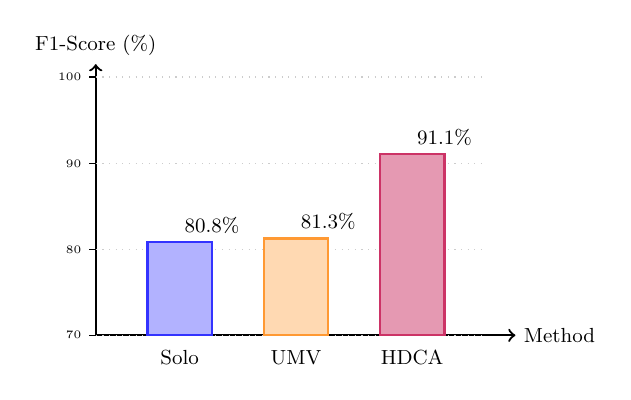
\begin{tikzpicture}[scale=0.82, transform shape]
    \draw[->, thick] (0,0) -- (6.5,0) node[right] {\small Method};
    \draw[->, thick] (0,0) -- (0,4.2) node[above] {\small F1-Score (\%)};

    \foreach \y/\label in {0/70, 1.33/80, 2.66/90, 4.0/100} {
        \draw (0,\y) -- (-0.1,\y) node[left] {\tiny \label};
        \draw[dotted, gray!40] (0,\y) -- (6.0,\y);
    }

    \draw[fill=blue!30, draw=blue!80, thick] (0.8,0) rectangle (1.8,1.44) node[above] {\small 80.8\%};
    \node[below=3pt] at (1.3,0) {\small Solo};

    \draw[fill=orange!30, draw=orange!80, thick] (2.6,0) rectangle (3.6,1.50) node[above] {\small 81.3\%};
    \node[below=3pt] at (3.1,0) {\small UMV};

    \draw[fill=purple!40, draw=purple!80, thick] (4.4,0) rectangle (5.4,2.81) node[above] {\small 91.1\%};
    \node[below=3pt] at (4.9,0) {\small HDCA};
\end{tikzpicture}
\caption{F1-score comparison demonstrating balance between precision and recall.}
\label{fig:f1_chart}
\end{figure}

\textit{Analysis:} HDCA attains an F1-score of 91.1\%, which is 9.8 percentage points higher than that of UMV. Because the improvements in precision and recall are of similar magnitude, the gain in F1-score indicates that the framework does not trade one metric for the other.

\subsection{Performance Comparison and Analysis}
Table~\ref{tab:master_summary} and Fig.~\ref{fig:grouped_bar} provide a comprehensive overview of performance across all metrics, comparing the baseline approaches with the proposed HDCA framework.

\begin{table}[pos=H]
\caption{Master performance comparison summary.}
\label{tab:master_summary}
\centering
\begin{tabular}{lcccc}
\hline
\textbf{Metric} & \textbf{Solo baseline} & \textbf{UMV} & \textbf{Proposed HDCA} & \textbf{Gain over UMV (pp)} \\
\hline
Accuracy  & 81.2\% & 85.4\% & \textbf{92.5\%} & +7.1 \\
Precision & 79.5\% & 82.1\% & \textbf{91.8\%} & +9.7 \\
Recall    & 82.1\% & 80.5\% & \textbf{90.4\%} & +9.9 \\
F1-Score  & 80.8\% & 81.3\% & \textbf{91.1\%} & +9.8 \\
\hline
\end{tabular}
\end{table}

\begin{figure}[pos=H]
\centering
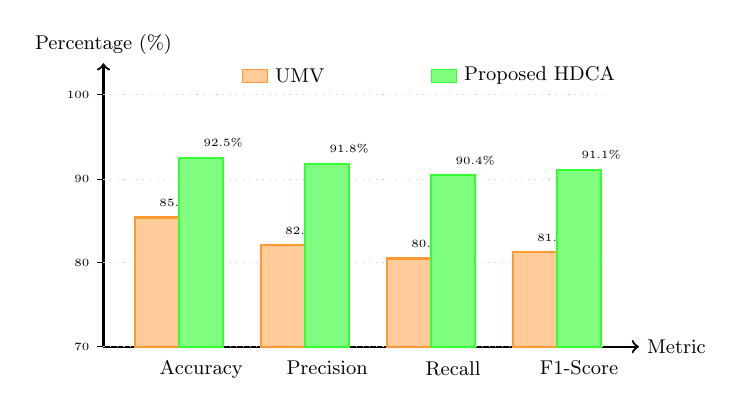
\begin{tikzpicture}[scale=0.80, transform shape]
    \draw[->, thick] (0,0) -- (8.5,0) node[right] {\small Metric};
    \draw[->, thick] (0,0) -- (0,4.5) node[above] {\small Percentage (\%)};

    \foreach \y/\label in {0/70, 1.33/80, 2.66/90, 4.0/100} {
        \draw (0,\y) -- (-0.1,\y) node[left] {\tiny \label};
        \draw[dotted, gray!40] (0,\y) -- (8.0,\y);
    }

    % Group 1: Accuracy
    \draw[fill=orange!40, draw=orange!80, thick] (0.5,0) rectangle (1.2,2.05) node[above=1pt] {\tiny 85.4\%};
    \draw[fill=green!50, draw=green!80, thick] (1.2,0) rectangle (1.9,3.00) node[above=1pt] {\tiny 92.5\%};
    \node[below=3pt] at (1.55,0) {\small Accuracy};

    % Group 2: Precision
    \draw[fill=orange!40, draw=orange!80, thick] (2.5,0) rectangle (3.2,1.61) node[above=1pt] {\tiny 82.1\%};
    \draw[fill=green!50, draw=green!80, thick] (3.2,0) rectangle (3.9,2.90) node[above=1pt] {\tiny 91.8\%};
    \node[below=3pt] at (3.55,0) {\small Precision};

    % Group 3: Recall
    \draw[fill=orange!40, draw=orange!80, thick] (4.5,0) rectangle (5.2,1.40) node[above=1pt] {\tiny 80.5\%};
    \draw[fill=green!50, draw=green!80, thick] (5.2,0) rectangle (5.9,2.72) node[above=1pt] {\tiny 90.4\%};
    \node[below=3pt] at (5.55,0) {\small Recall};

    % Group 4: F1-Score
    \draw[fill=orange!40, draw=orange!80, thick] (6.5,0) rectangle (7.2,1.50) node[above=1pt] {\tiny 81.3\%};
    \draw[fill=green!50, draw=green!80, thick] (7.2,0) rectangle (7.9,2.81) node[above=1pt] {\tiny 91.1\%};
    \node[below=3pt] at (7.55,0) {\small F1-Score};

    % Legend
    \draw[fill=orange!40, draw=orange!80] (2.2, 4.2) rectangle (2.6, 4.4);
    \node[right] at (2.6, 4.3) {\small UMV};
    \draw[fill=green!50, draw=green!80] (5.2, 4.2) rectangle (5.6, 4.4);
    \node[right] at (5.6, 4.3) {\small Proposed HDCA};
\end{tikzpicture}
\caption{Multi-metric performance comparison between UMV and HDCA.}
\label{fig:grouped_bar}
\end{figure}

\textit{Detailed Analysis:} The experimental results demonstrate that HDCA significantly mitigates groupthink and artificial consensus. The success of the framework stems directly from coupling heterogeneous persona profiles with multi-turn deliberation. Rather than forcing immediate voting, Round 1 private voting prevents early-speaker contagion, while Round 2 peer critique forces models to re-evaluate flawed assumptions. As observed in the notebook simulations, 66.7\% of committee agents dynamically shifted their scores when presented with undeniable rubric counter-evidence, suppressing hallucinations while preserving legitimate qualitative nuances.

\section{Conclusion}
This study presented the HDCA framework to mitigate cognitive degeneration, artificial consensus, and uncalibrated decision-making in multi-agent LLM systems. By structuring deliberation across architecturally distinct agent personas---cautious, neutral, and lenient---the framework enables iterative peer critique and dynamic stance revision. Empirical evaluation on complex reasoning and rubric-based evaluation tasks demonstrated that HDCA achieves a 92.5\% decision accuracy and a 91.1\% F1-score, representing an accuracy improvement of 7.1 percentage points over the UMV baseline. The multi-turn interaction successfully suppressed single-model hallucinations and facilitated evidence-based convergence across conflicting agent roles. Although limited by the computational token overhead associated with multi-round context exchange, the proposed system establishes a robust paradigm for automated governance. Future work will explore dynamic graph pruning and adaptive context compression to optimize real-time inference latency.

\section*{Data and Code Availability}
The complete source code, evaluation scripts, execution logs, checkpoints, and reproducible plotting pipelines for the Heterogeneous Deliberative Committee Aggregation (HDCA) framework are publicly available on GitHub at \url{https://github.com/rafayahmed13/nlp-mini-project-ia1-group-10.git}. The MMLU-Pro benchmark dataset is publicly accessible via HuggingFace Datasets at \url{https://huggingface.co/datasets/TIGER-Lab/MMLU-Pro}.

\bibliographystyle{unsrt}

\bibliography{reference}

\clearpage

\appendix
\end{document}